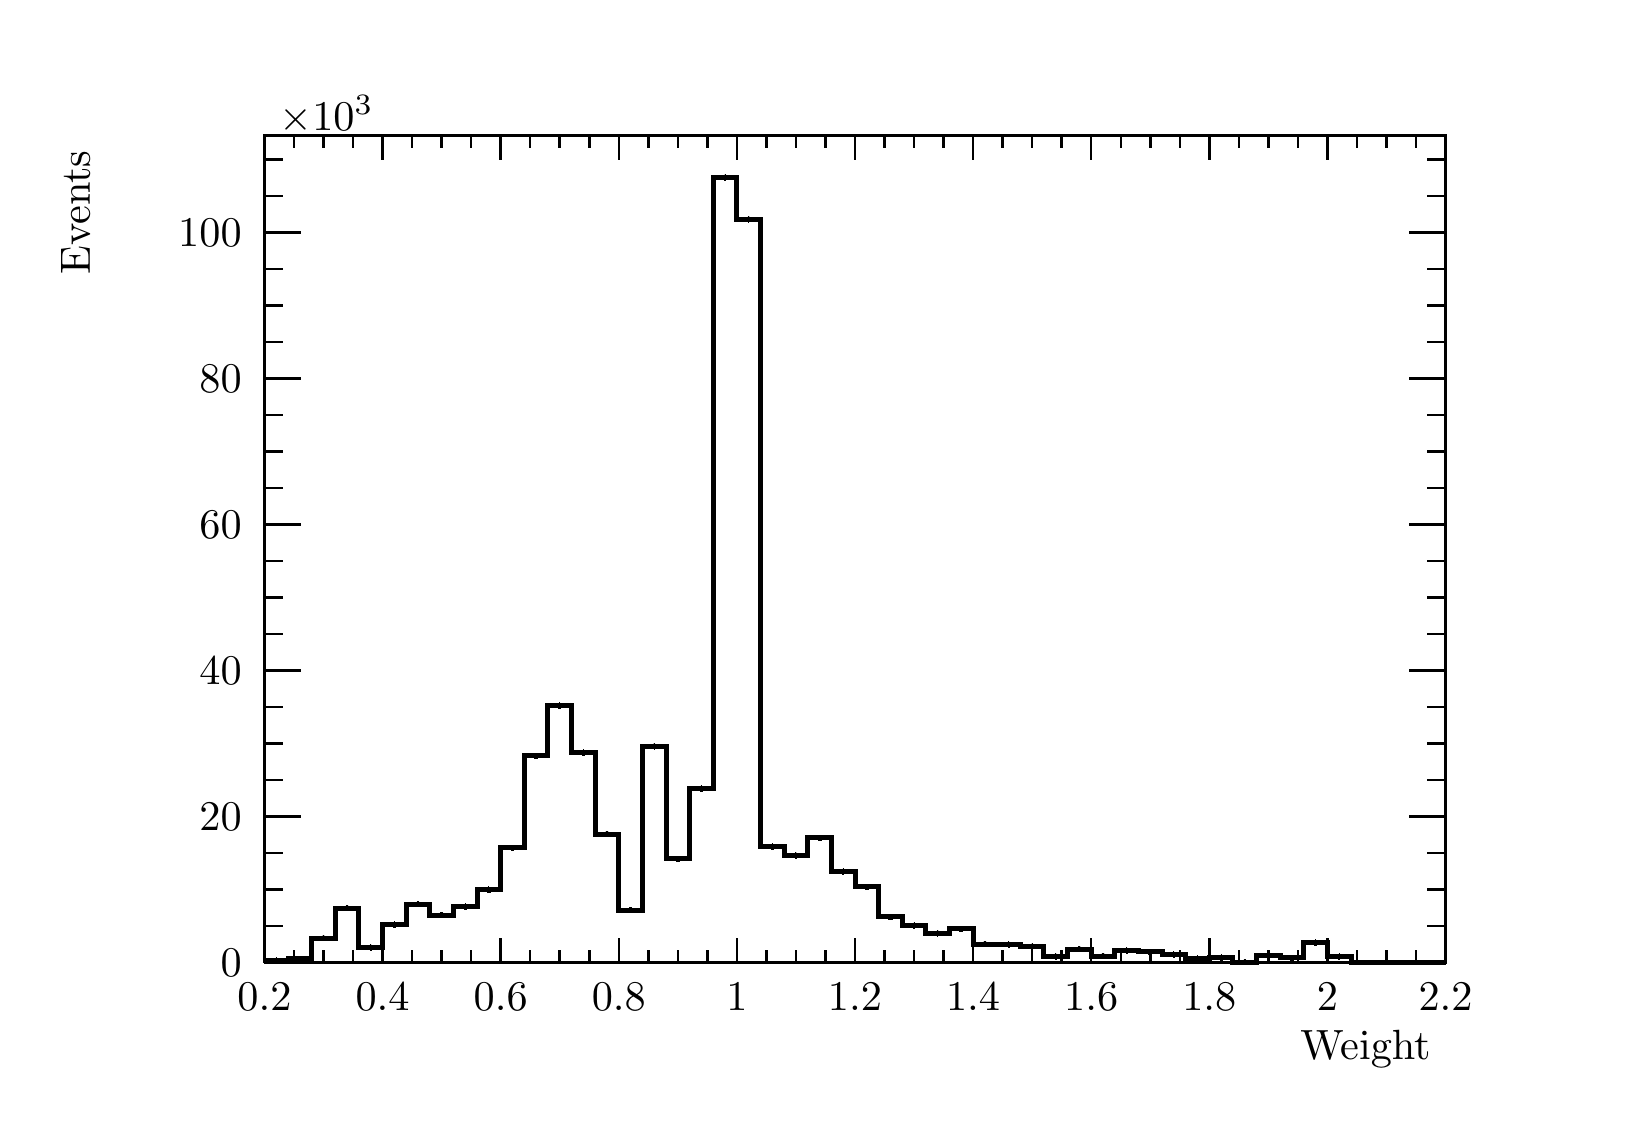
\begin{tikzpicture}
\pgfdeclareplotmark{cross} {
\pgfpathmoveto{\pgfpoint{-0.3\pgfplotmarksize}{\pgfplotmarksize}}
\pgfpathlineto{\pgfpoint{+0.3\pgfplotmarksize}{\pgfplotmarksize}}
\pgfpathlineto{\pgfpoint{+0.3\pgfplotmarksize}{0.3\pgfplotmarksize}}
\pgfpathlineto{\pgfpoint{+1\pgfplotmarksize}{0.3\pgfplotmarksize}}
\pgfpathlineto{\pgfpoint{+1\pgfplotmarksize}{-0.3\pgfplotmarksize}}
\pgfpathlineto{\pgfpoint{+0.3\pgfplotmarksize}{-0.3\pgfplotmarksize}}
\pgfpathlineto{\pgfpoint{+0.3\pgfplotmarksize}{-1.\pgfplotmarksize}}
\pgfpathlineto{\pgfpoint{-0.3\pgfplotmarksize}{-1.\pgfplotmarksize}}
\pgfpathlineto{\pgfpoint{-0.3\pgfplotmarksize}{-0.3\pgfplotmarksize}}
\pgfpathlineto{\pgfpoint{-1.\pgfplotmarksize}{-0.3\pgfplotmarksize}}
\pgfpathlineto{\pgfpoint{-1.\pgfplotmarksize}{0.3\pgfplotmarksize}}
\pgfpathlineto{\pgfpoint{-0.3\pgfplotmarksize}{0.3\pgfplotmarksize}}
\pgfpathclose
\pgfusepathqstroke
}
\pgfdeclareplotmark{cross*} {
\pgfpathmoveto{\pgfpoint{-0.3\pgfplotmarksize}{\pgfplotmarksize}}
\pgfpathlineto{\pgfpoint{+0.3\pgfplotmarksize}{\pgfplotmarksize}}
\pgfpathlineto{\pgfpoint{+0.3\pgfplotmarksize}{0.3\pgfplotmarksize}}
\pgfpathlineto{\pgfpoint{+1\pgfplotmarksize}{0.3\pgfplotmarksize}}
\pgfpathlineto{\pgfpoint{+1\pgfplotmarksize}{-0.3\pgfplotmarksize}}
\pgfpathlineto{\pgfpoint{+0.3\pgfplotmarksize}{-0.3\pgfplotmarksize}}
\pgfpathlineto{\pgfpoint{+0.3\pgfplotmarksize}{-1.\pgfplotmarksize}}
\pgfpathlineto{\pgfpoint{-0.3\pgfplotmarksize}{-1.\pgfplotmarksize}}
\pgfpathlineto{\pgfpoint{-0.3\pgfplotmarksize}{-0.3\pgfplotmarksize}}
\pgfpathlineto{\pgfpoint{-1.\pgfplotmarksize}{-0.3\pgfplotmarksize}}
\pgfpathlineto{\pgfpoint{-1.\pgfplotmarksize}{0.3\pgfplotmarksize}}
\pgfpathlineto{\pgfpoint{-0.3\pgfplotmarksize}{0.3\pgfplotmarksize}}
\pgfpathclose
\pgfusepathqfillstroke
}
\pgfdeclareplotmark{newstar} {
\pgfpathmoveto{\pgfqpoint{0pt}{\pgfplotmarksize}}
\pgfpathlineto{\pgfqpointpolar{44}{0.5\pgfplotmarksize}}
\pgfpathlineto{\pgfqpointpolar{18}{\pgfplotmarksize}}
\pgfpathlineto{\pgfqpointpolar{-20}{0.5\pgfplotmarksize}}
\pgfpathlineto{\pgfqpointpolar{-54}{\pgfplotmarksize}}
\pgfpathlineto{\pgfqpointpolar{-90}{0.5\pgfplotmarksize}}
\pgfpathlineto{\pgfqpointpolar{234}{\pgfplotmarksize}}
\pgfpathlineto{\pgfqpointpolar{198}{0.5\pgfplotmarksize}}
\pgfpathlineto{\pgfqpointpolar{162}{\pgfplotmarksize}}
\pgfpathlineto{\pgfqpointpolar{134}{0.5\pgfplotmarksize}}
\pgfpathclose
\pgfusepathqstroke
}
\pgfdeclareplotmark{newstar*} {
\pgfpathmoveto{\pgfqpoint{0pt}{\pgfplotmarksize}}
\pgfpathlineto{\pgfqpointpolar{44}{0.5\pgfplotmarksize}}
\pgfpathlineto{\pgfqpointpolar{18}{\pgfplotmarksize}}
\pgfpathlineto{\pgfqpointpolar{-20}{0.5\pgfplotmarksize}}
\pgfpathlineto{\pgfqpointpolar{-54}{\pgfplotmarksize}}
\pgfpathlineto{\pgfqpointpolar{-90}{0.5\pgfplotmarksize}}
\pgfpathlineto{\pgfqpointpolar{234}{\pgfplotmarksize}}
\pgfpathlineto{\pgfqpointpolar{198}{0.5\pgfplotmarksize}}
\pgfpathlineto{\pgfqpointpolar{162}{\pgfplotmarksize}}
\pgfpathlineto{\pgfqpointpolar{134}{0.5\pgfplotmarksize}}
\pgfpathclose
\pgfusepathqfillstroke
}
\definecolor{c}{rgb}{1,1,1};
\draw [color=c, fill=c] (0,0) rectangle (20,13.639);
\draw [color=c, fill=c] (3,1.77307) rectangle (18,12.2751);
\definecolor{c}{rgb}{0,0,0};
\draw [c,line width=0.9] (3,1.77307) -- (3,12.2751) -- (18,12.2751) -- (18,1.77307) -- (3,1.77307);
\definecolor{c}{rgb}{1,1,1};
\draw [color=c, fill=c] (3,1.77307) rectangle (18,12.2751);
\definecolor{c}{rgb}{0,0,0};
\draw [c,line width=0.9] (3,1.77307) -- (3,12.2751) -- (18,12.2751) -- (18,1.77307) -- (3,1.77307);
\draw [c,line width=1.8] (3.15,1.79585) -- (3.15,1.79735);
\draw [c,line width=1.8] (3.15,1.79735) -- (3.15,1.79885);
\foreach \P in {(3.15,1.79735)}{\draw[mark options={color=c,fill=c},mark size=2.402402pt, line width=0.000000pt, mark=*,mark size=1pt] plot coordinates {\P};}
\draw [c,line width=1.8] (3.45,1.81889) -- (3.45,1.82099);
\draw [c,line width=1.8] (3.45,1.82099) -- (3.45,1.8231);
\foreach \P in {(3.45,1.82099)}{\draw[mark options={color=c,fill=c},mark size=2.402402pt, line width=0.000000pt, mark=*,mark size=1pt] plot coordinates {\P};}
\draw [c,line width=1.8] (3.75,2.07706) -- (3.75,2.08241);
\draw [c,line width=1.8] (3.75,2.08241) -- (3.75,2.08777);
\foreach \P in {(3.75,2.08241)}{\draw[mark options={color=c,fill=c},mark size=2.402402pt, line width=0.000000pt, mark=*,mark size=1pt] plot coordinates {\P};}
\draw [c,line width=1.8] (4.05,2.45662) -- (4.05,2.46462);
\draw [c,line width=1.8] (4.05,2.46462) -- (4.05,2.47263);
\foreach \P in {(4.05,2.46462)}{\draw[mark options={color=c,fill=c},mark size=2.402402pt, line width=0.000000pt, mark=*,mark size=1pt] plot coordinates {\P};}
\draw [c,line width=1.8] (4.35,1.96148) -- (4.35,1.9657);
\draw [c,line width=1.8] (4.35,1.9657) -- (4.35,1.96993);
\foreach \P in {(4.35,1.9657)}{\draw[mark options={color=c,fill=c},mark size=2.402402pt, line width=0.000000pt, mark=*,mark size=1pt] plot coordinates {\P};}
\draw [c,line width=1.8] (4.65,2.24751) -- (4.65,2.25419);
\draw [c,line width=1.8] (4.65,2.25419) -- (4.65,2.26087);
\foreach \P in {(4.65,2.25419)}{\draw[mark options={color=c,fill=c},mark size=2.402402pt, line width=0.000000pt, mark=*,mark size=1pt] plot coordinates {\P};}
\draw [c,line width=1.8] (4.95,2.50602) -- (4.95,2.51431);
\draw [c,line width=1.8] (4.95,2.51431) -- (4.95,2.5226);
\foreach \P in {(4.95,2.51431)}{\draw[mark options={color=c,fill=c},mark size=2.402402pt, line width=0.000000pt, mark=*,mark size=1pt] plot coordinates {\P};}
\draw [c,line width=1.8] (5.25,2.3688) -- (5.25,2.37628);
\draw [c,line width=1.8] (5.25,2.37628) -- (5.25,2.38376);
\foreach \P in {(5.25,2.37628)}{\draw[mark options={color=c,fill=c},mark size=2.402402pt, line width=0.000000pt, mark=*,mark size=1pt] plot coordinates {\P};}
\draw [c,line width=1.8] (5.55,2.47422) -- (5.55,2.48233);
\draw [c,line width=1.8] (5.55,2.48233) -- (5.55,2.49044);
\foreach \P in {(5.55,2.48233)}{\draw[mark options={color=c,fill=c},mark size=2.402402pt, line width=0.000000pt, mark=*,mark size=1pt] plot coordinates {\P};}
\draw [c,line width=1.8] (5.85,2.6887) -- (5.85,2.69796);
\draw [c,line width=1.8] (5.85,2.69796) -- (5.85,2.70721);
\foreach \P in {(5.85,2.69796)}{\draw[mark options={color=c,fill=c},mark size=2.402402pt, line width=0.000000pt, mark=*,mark size=1pt] plot coordinates {\P};}
\draw [c,line width=1.8] (6.15,3.21891) -- (6.15,3.23053);
\draw [c,line width=1.8] (6.15,3.23053) -- (6.15,3.24215);
\foreach \P in {(6.15,3.23053)}{\draw[mark options={color=c,fill=c},mark size=2.402402pt, line width=0.000000pt, mark=*,mark size=1pt] plot coordinates {\P};}
\draw [c,line width=1.8] (6.45,4.38214) -- (6.45,4.39774);
\draw [c,line width=1.8] (6.45,4.39774) -- (6.45,4.41334);
\foreach \P in {(6.45,4.39774)}{\draw[mark options={color=c,fill=c},mark size=2.402402pt, line width=0.000000pt, mark=*,mark size=1pt] plot coordinates {\P};}
\draw [c,line width=1.8] (6.75,5.01851) -- (6.75,5.0359);
\draw [c,line width=1.8] (6.75,5.0359) -- (6.75,5.0533);
\foreach \P in {(6.75,5.0359)}{\draw[mark options={color=c,fill=c},mark size=2.402402pt, line width=0.000000pt, mark=*,mark size=1pt] plot coordinates {\P};}
\draw [c,line width=1.8] (7.05,4.42281) -- (7.05,4.43853);
\draw [c,line width=1.8] (7.05,4.43853) -- (7.05,4.45425);
\foreach \P in {(7.05,4.43853)}{\draw[mark options={color=c,fill=c},mark size=2.402402pt, line width=0.000000pt, mark=*,mark size=1pt] plot coordinates {\P};}
\draw [c,line width=1.8] (7.35,3.39316) -- (7.35,3.40546);
\draw [c,line width=1.8] (7.35,3.40546) -- (7.35,3.41776);
\foreach \P in {(7.35,3.40546)}{\draw[mark options={color=c,fill=c},mark size=2.402402pt, line width=0.000000pt, mark=*,mark size=1pt] plot coordinates {\P};}
\draw [c,line width=1.8] (7.65,2.43137) -- (7.65,2.43922);
\draw [c,line width=1.8] (7.65,2.43922) -- (7.65,2.44708);
\foreach \P in {(7.65,2.43922)}{\draw[mark options={color=c,fill=c},mark size=2.402402pt, line width=0.000000pt, mark=*,mark size=1pt] plot coordinates {\P};}
\draw [c,line width=1.8] (7.95,4.50378) -- (7.95,4.51974);
\draw [c,line width=1.8] (7.95,4.51974) -- (7.95,4.53569);
\foreach \P in {(7.95,4.51974)}{\draw[mark options={color=c,fill=c},mark size=2.402402pt, line width=0.000000pt, mark=*,mark size=1pt] plot coordinates {\P};}
\draw [c,line width=1.8] (8.25,3.07922) -- (8.25,3.09027);
\draw [c,line width=1.8] (8.25,3.09027) -- (8.25,3.10132);
\foreach \P in {(8.25,3.09027)}{\draw[mark options={color=c,fill=c},mark size=2.402402pt, line width=0.000000pt, mark=*,mark size=1pt] plot coordinates {\P};}
\draw [c,line width=1.8] (8.55,3.9696) -- (8.55,3.98392);
\draw [c,line width=1.8] (8.55,3.98392) -- (8.55,3.99824);
\foreach \P in {(8.55,3.98392)}{\draw[mark options={color=c,fill=c},mark size=2.402402pt, line width=0.000000pt, mark=*,mark size=1pt] plot coordinates {\P};}
\draw [c,line width=1.8] (8.85,11.7142) -- (8.85,11.7446);
\draw [c,line width=1.8] (8.85,11.7446) -- (8.85,11.775);
\foreach \P in {(8.85,11.7446)}{\draw[mark options={color=c,fill=c},mark size=2.402402pt, line width=0.000000pt, mark=*,mark size=1pt] plot coordinates {\P};}
\draw [c,line width=1.8] (9.15,11.1829) -- (9.15,11.2125);
\draw [c,line width=1.8] (9.15,11.2125) -- (9.15,11.242);
\foreach \P in {(9.15,11.2125)}{\draw[mark options={color=c,fill=c},mark size=2.402402pt, line width=0.000000pt, mark=*,mark size=1pt] plot coordinates {\P};}
\draw [c,line width=1.8] (9.45,3.23368) -- (9.45,3.24536);
\draw [c,line width=1.8] (9.45,3.24536) -- (9.45,3.25704);
\foreach \P in {(9.45,3.24536)}{\draw[mark options={color=c,fill=c},mark size=2.402402pt, line width=0.000000pt, mark=*,mark size=1pt] plot coordinates {\P};}
\draw [c,line width=1.8] (9.75,3.12289) -- (9.75,3.13412);
\draw [c,line width=1.8] (9.75,3.13412) -- (9.75,3.14535);
\foreach \P in {(9.75,3.13412)}{\draw[mark options={color=c,fill=c},mark size=2.402402pt, line width=0.000000pt, mark=*,mark size=1pt] plot coordinates {\P};}
\draw [c,line width=1.8] (10.05,3.34449) -- (10.05,3.3566);
\draw [c,line width=1.8] (10.05,3.3566) -- (10.05,3.36872);
\foreach \P in {(10.05,3.3566)}{\draw[mark options={color=c,fill=c},mark size=2.402402pt, line width=0.000000pt, mark=*,mark size=1pt] plot coordinates {\P};}
\draw [c,line width=1.8] (10.35,2.91899) -- (10.35,2.92934);
\draw [c,line width=1.8] (10.35,2.92934) -- (10.35,2.93969);
\foreach \P in {(10.35,2.92934)}{\draw[mark options={color=c,fill=c},mark size=2.402402pt, line width=0.000000pt, mark=*,mark size=1pt] plot coordinates {\P};}
\draw [c,line width=1.8] (10.65,2.72449) -- (10.65,2.73392);
\draw [c,line width=1.8] (10.65,2.73392) -- (10.65,2.74336);
\foreach \P in {(10.65,2.73392)}{\draw[mark options={color=c,fill=c},mark size=2.402402pt, line width=0.000000pt, mark=*,mark size=1pt] plot coordinates {\P};}
\draw [c,line width=1.8] (10.95,2.34476) -- (10.95,2.35208);
\draw [c,line width=1.8] (10.95,2.35208) -- (10.95,2.35941);
\foreach \P in {(10.95,2.35208)}{\draw[mark options={color=c,fill=c},mark size=2.402402pt, line width=0.000000pt, mark=*,mark size=1pt] plot coordinates {\P};}
\draw [c,line width=1.8] (11.25,2.23711) -- (11.25,2.24371);
\draw [c,line width=1.8] (11.25,2.24371) -- (11.25,2.25032);
\foreach \P in {(11.25,2.24371)}{\draw[mark options={color=c,fill=c},mark size=2.402402pt, line width=0.000000pt, mark=*,mark size=1pt] plot coordinates {\P};}
\draw [c,line width=1.8] (11.55,2.13838) -- (11.55,2.14425);
\draw [c,line width=1.8] (11.55,2.14425) -- (11.55,2.15011);
\foreach \P in {(11.55,2.14425)}{\draw[mark options={color=c,fill=c},mark size=2.402402pt, line width=0.000000pt, mark=*,mark size=1pt] plot coordinates {\P};}
\draw [c,line width=1.8] (11.85,2.1956) -- (11.85,2.20191);
\draw [c,line width=1.8] (11.85,2.20191) -- (11.85,2.20821);
\foreach \P in {(11.85,2.20191)}{\draw[mark options={color=c,fill=c},mark size=2.402402pt, line width=0.000000pt, mark=*,mark size=1pt] plot coordinates {\P};}
\draw [c,line width=1.8] (12.15,2.00321) -- (12.15,2.00788);
\draw [c,line width=1.8] (12.15,2.00788) -- (12.15,2.01255);
\foreach \P in {(12.15,2.00788)}{\draw[mark options={color=c,fill=c},mark size=2.402402pt, line width=0.000000pt, mark=*,mark size=1pt] plot coordinates {\P};}
\draw [c,line width=1.8] (12.45,1.99835) -- (12.45,2.00297);
\draw [c,line width=1.8] (12.45,2.00297) -- (12.45,2.00758);
\foreach \P in {(12.45,2.00297)}{\draw[mark options={color=c,fill=c},mark size=2.402402pt, line width=0.000000pt, mark=*,mark size=1pt] plot coordinates {\P};}
\draw [c,line width=1.8] (12.75,1.97413) -- (12.75,1.97849);
\draw [c,line width=1.8] (12.75,1.97849) -- (12.75,1.98286);
\foreach \P in {(12.75,1.97849)}{\draw[mark options={color=c,fill=c},mark size=2.402402pt, line width=0.000000pt, mark=*,mark size=1pt] plot coordinates {\P};}
\draw [c,line width=1.8] (13.05,1.84816) -- (13.05,1.85084);
\draw [c,line width=1.8] (13.05,1.85084) -- (13.05,1.85353);
\foreach \P in {(13.05,1.85084)}{\draw[mark options={color=c,fill=c},mark size=2.402402pt, line width=0.000000pt, mark=*,mark size=1pt] plot coordinates {\P};}
\draw [c,line width=1.8] (13.35,1.93902) -- (13.35,1.94299);
\draw [c,line width=1.8] (13.35,1.94299) -- (13.35,1.94696);
\foreach \P in {(13.35,1.94299)}{\draw[mark options={color=c,fill=c},mark size=2.402402pt, line width=0.000000pt, mark=*,mark size=1pt] plot coordinates {\P};}
\draw [c,line width=1.8] (13.65,1.85308) -- (13.65,1.85585);
\draw [c,line width=1.8] (13.65,1.85585) -- (13.65,1.85862);
\foreach \P in {(13.65,1.85585)}{\draw[mark options={color=c,fill=c},mark size=2.402402pt, line width=0.000000pt, mark=*,mark size=1pt] plot coordinates {\P};}
\draw [c,line width=1.8] (13.95,1.92244) -- (13.95,1.92621);
\draw [c,line width=1.8] (13.95,1.92621) -- (13.95,1.92998);
\foreach \P in {(13.95,1.92621)}{\draw[mark options={color=c,fill=c},mark size=2.402402pt, line width=0.000000pt, mark=*,mark size=1pt] plot coordinates {\P};}
\draw [c,line width=1.8] (14.25,1.90542) -- (14.25,1.90897);
\draw [c,line width=1.8] (14.25,1.90897) -- (14.25,1.91252);
\foreach \P in {(14.25,1.90897)}{\draw[mark options={color=c,fill=c},mark size=2.402402pt, line width=0.000000pt, mark=*,mark size=1pt] plot coordinates {\P};}
\draw [c,line width=1.8] (14.55,1.87123) -- (14.55,1.8743);
\draw [c,line width=1.8] (14.55,1.8743) -- (14.55,1.87736);
\foreach \P in {(14.55,1.8743)}{\draw[mark options={color=c,fill=c},mark size=2.402402pt, line width=0.000000pt, mark=*,mark size=1pt] plot coordinates {\P};}
\draw [c,line width=1.8] (14.85,1.81988) -- (14.85,1.82201);
\draw [c,line width=1.8] (14.85,1.82201) -- (14.85,1.82414);
\foreach \P in {(14.85,1.82201)}{\draw[mark options={color=c,fill=c},mark size=2.402402pt, line width=0.000000pt, mark=*,mark size=1pt] plot coordinates {\P};}
\draw [c,line width=1.8] (15.15,1.83314) -- (15.15,1.83555);
\draw [c,line width=1.8] (15.15,1.83555) -- (15.15,1.83795);
\foreach \P in {(15.15,1.83555)}{\draw[mark options={color=c,fill=c},mark size=2.402402pt, line width=0.000000pt, mark=*,mark size=1pt] plot coordinates {\P};}
\draw [c,line width=1.8] (15.45,1.7767) -- (15.45,1.77733);
\draw [c,line width=1.8] (15.45,1.77733) -- (15.45,1.77796);
\foreach \P in {(15.45,1.77733)}{\draw[mark options={color=c,fill=c},mark size=2.402402pt, line width=0.000000pt, mark=*,mark size=1pt] plot coordinates {\P};}
\draw [c,line width=1.8] (15.75,1.86147) -- (15.75,1.86438);
\draw [c,line width=1.8] (15.75,1.86438) -- (15.75,1.86729);
\foreach \P in {(15.75,1.86438)}{\draw[mark options={color=c,fill=c},mark size=2.402402pt, line width=0.000000pt, mark=*,mark size=1pt] plot coordinates {\P};}
\draw [c,line width=1.8] (16.05,1.82887) -- (16.05,1.83119);
\draw [c,line width=1.8] (16.05,1.83119) -- (16.05,1.83351);
\foreach \P in {(16.05,1.83119)}{\draw[mark options={color=c,fill=c},mark size=2.402402pt, line width=0.000000pt, mark=*,mark size=1pt] plot coordinates {\P};}
\draw [c,line width=1.8] (16.35,2.02112) -- (16.35,2.02596);
\draw [c,line width=1.8] (16.35,2.02596) -- (16.35,2.0308);
\foreach \P in {(16.35,2.02596)}{\draw[mark options={color=c,fill=c},mark size=2.402402pt, line width=0.000000pt, mark=*,mark size=1pt] plot coordinates {\P};}
\draw [c,line width=1.8] (16.65,1.84716) -- (16.65,1.84982);
\draw [c,line width=1.8] (16.65,1.84982) -- (16.65,1.85249);
\foreach \P in {(16.65,1.84982)}{\draw[mark options={color=c,fill=c},mark size=2.402402pt, line width=0.000000pt, mark=*,mark size=1pt] plot coordinates {\P};}
\draw [c,line width=1.8] (3,1.79735) -- (3.3,1.79735) -- (3.3,1.82099) -- (3.6,1.82099) -- (3.6,2.08241) -- (3.9,2.08241) -- (3.9,2.46462) -- (4.2,2.46462) -- (4.2,1.9657) -- (4.5,1.9657) -- (4.5,2.25419) -- (4.8,2.25419) -- (4.8,2.51431) --
 (5.1,2.51431) -- (5.1,2.37628) -- (5.4,2.37628) -- (5.4,2.48233) -- (5.7,2.48233) -- (5.7,2.69796) -- (6,2.69796) -- (6,3.23053) -- (6.3,3.23053) -- (6.3,4.39774) -- (6.6,4.39774) -- (6.6,5.0359) -- (6.9,5.0359) -- (6.9,4.43853) -- (7.2,4.43853) --
 (7.2,3.40546) -- (7.5,3.40546) -- (7.5,2.43922) -- (7.8,2.43922) -- (7.8,4.51974) -- (8.1,4.51974) -- (8.1,3.09027) -- (8.4,3.09027) -- (8.4,3.98392) -- (8.7,3.98392) -- (8.7,11.7446) -- (9,11.7446) -- (9,11.2125) -- (9.3,11.2125) -- (9.3,3.24536)
 -- (9.6,3.24536) -- (9.6,3.13412) -- (9.9,3.13412) -- (9.9,3.3566) -- (10.2,3.3566) -- (10.2,2.92934) -- (10.5,2.92934) -- (10.5,2.73392) -- (10.8,2.73392) -- (10.8,2.35208) -- (11.1,2.35208) -- (11.1,2.24371) -- (11.4,2.24371) -- (11.4,2.14425) --
 (11.7,2.14425) -- (11.7,2.20191) -- (12,2.20191) -- (12,2.00788) -- (12.3,2.00788) -- (12.3,2.00297) -- (12.6,2.00297) -- (12.6,1.97849) -- (12.9,1.97849) -- (12.9,1.85084) -- (13.2,1.85084) -- (13.2,1.94299) -- (13.5,1.94299) -- (13.5,1.85585) --
 (13.8,1.85585) -- (13.8,1.92621) -- (14.1,1.92621) -- (14.1,1.90897) -- (14.4,1.90897) -- (14.4,1.8743) -- (14.7,1.8743) -- (14.7,1.82201) -- (15,1.82201) -- (15,1.83555) -- (15.3,1.83555) -- (15.3,1.77733) -- (15.6,1.77733) -- (15.6,1.86438) --
 (15.9,1.86438) -- (15.9,1.83119) -- (16.2,1.83119) -- (16.2,2.02596) -- (16.5,2.02596) -- (16.5,1.84982) -- (16.8,1.84982) -- (16.8,1.77307) -- (17.1,1.77307) -- (17.1,1.77307) -- (17.4,1.77307) -- (17.4,1.77307) -- (17.7,1.77307) -- (17.7,1.77307)
 -- (18,1.77307);
\draw [c,line width=0.9] (3,1.77307) -- (18,1.77307);
\draw [c,line width=0.9] (3,2.07994) -- (3,1.77307);
\draw [c,line width=0.9] (3.375,1.9265) -- (3.375,1.77307);
\draw [c,line width=0.9] (3.75,1.9265) -- (3.75,1.77307);
\draw [c,line width=0.9] (4.125,1.9265) -- (4.125,1.77307);
\draw [c,line width=0.9] (4.5,2.07994) -- (4.5,1.77307);
\draw [c,line width=0.9] (4.875,1.9265) -- (4.875,1.77307);
\draw [c,line width=0.9] (5.25,1.9265) -- (5.25,1.77307);
\draw [c,line width=0.9] (5.625,1.9265) -- (5.625,1.77307);
\draw [c,line width=0.9] (6,2.07994) -- (6,1.77307);
\draw [c,line width=0.9] (6.375,1.9265) -- (6.375,1.77307);
\draw [c,line width=0.9] (6.75,1.9265) -- (6.75,1.77307);
\draw [c,line width=0.9] (7.125,1.9265) -- (7.125,1.77307);
\draw [c,line width=0.9] (7.5,2.07994) -- (7.5,1.77307);
\draw [c,line width=0.9] (7.875,1.9265) -- (7.875,1.77307);
\draw [c,line width=0.9] (8.25,1.9265) -- (8.25,1.77307);
\draw [c,line width=0.9] (8.625,1.9265) -- (8.625,1.77307);
\draw [c,line width=0.9] (9,2.07994) -- (9,1.77307);
\draw [c,line width=0.9] (9.375,1.9265) -- (9.375,1.77307);
\draw [c,line width=0.9] (9.75,1.9265) -- (9.75,1.77307);
\draw [c,line width=0.9] (10.125,1.9265) -- (10.125,1.77307);
\draw [c,line width=0.9] (10.5,2.07994) -- (10.5,1.77307);
\draw [c,line width=0.9] (10.875,1.9265) -- (10.875,1.77307);
\draw [c,line width=0.9] (11.25,1.9265) -- (11.25,1.77307);
\draw [c,line width=0.9] (11.625,1.9265) -- (11.625,1.77307);
\draw [c,line width=0.9] (12,2.07994) -- (12,1.77307);
\draw [c,line width=0.9] (12.375,1.9265) -- (12.375,1.77307);
\draw [c,line width=0.9] (12.75,1.9265) -- (12.75,1.77307);
\draw [c,line width=0.9] (13.125,1.9265) -- (13.125,1.77307);
\draw [c,line width=0.9] (13.5,2.07994) -- (13.5,1.77307);
\draw [c,line width=0.9] (13.875,1.9265) -- (13.875,1.77307);
\draw [c,line width=0.9] (14.25,1.9265) -- (14.25,1.77307);
\draw [c,line width=0.9] (14.625,1.9265) -- (14.625,1.77307);
\draw [c,line width=0.9] (15,2.07994) -- (15,1.77307);
\draw [c,line width=0.9] (15.375,1.9265) -- (15.375,1.77307);
\draw [c,line width=0.9] (15.75,1.9265) -- (15.75,1.77307);
\draw [c,line width=0.9] (16.125,1.9265) -- (16.125,1.77307);
\draw [c,line width=0.9] (16.5,2.07994) -- (16.5,1.77307);
\draw [c,line width=0.9] (16.875,1.9265) -- (16.875,1.77307);
\draw [c,line width=0.9] (17.25,1.9265) -- (17.25,1.77307);
\draw [c,line width=0.9] (17.625,1.9265) -- (17.625,1.77307);
\draw [c,line width=0.9] (18,2.07994) -- (18,1.77307);
\draw [anchor=base] (3,1.15931) node[scale=1.52731, color=c, rotate=0]{0.2};
\draw [anchor=base] (4.5,1.15931) node[scale=1.52731, color=c, rotate=0]{0.4};
\draw [anchor=base] (6,1.15931) node[scale=1.52731, color=c, rotate=0]{0.6};
\draw [anchor=base] (7.5,1.15931) node[scale=1.52731, color=c, rotate=0]{0.8};
\draw [anchor=base] (9,1.15931) node[scale=1.52731, color=c, rotate=0]{1};
\draw [anchor=base] (10.5,1.15931) node[scale=1.52731, color=c, rotate=0]{1.2};
\draw [anchor=base] (12,1.15931) node[scale=1.52731, color=c, rotate=0]{1.4};
\draw [anchor=base] (13.5,1.15931) node[scale=1.52731, color=c, rotate=0]{1.6};
\draw [anchor=base] (15,1.15931) node[scale=1.52731, color=c, rotate=0]{1.8};
\draw [anchor=base] (16.5,1.15931) node[scale=1.52731, color=c, rotate=0]{2};
\draw [anchor=base] (18,1.15931) node[scale=1.52731, color=c, rotate=0]{2.2};
\draw [anchor= east] (18,0.681948) node[scale=1.52731, color=c, rotate=0]{ Weight};
\draw [c,line width=0.9] (3,12.2751) -- (18,12.2751);
\draw [c,line width=0.9] (3,11.9682) -- (3,12.2751);
\draw [c,line width=0.9] (3.375,12.1216) -- (3.375,12.2751);
\draw [c,line width=0.9] (3.75,12.1216) -- (3.75,12.2751);
\draw [c,line width=0.9] (4.125,12.1216) -- (4.125,12.2751);
\draw [c,line width=0.9] (4.5,11.9682) -- (4.5,12.2751);
\draw [c,line width=0.9] (4.875,12.1216) -- (4.875,12.2751);
\draw [c,line width=0.9] (5.25,12.1216) -- (5.25,12.2751);
\draw [c,line width=0.9] (5.625,12.1216) -- (5.625,12.2751);
\draw [c,line width=0.9] (6,11.9682) -- (6,12.2751);
\draw [c,line width=0.9] (6.375,12.1216) -- (6.375,12.2751);
\draw [c,line width=0.9] (6.75,12.1216) -- (6.75,12.2751);
\draw [c,line width=0.9] (7.125,12.1216) -- (7.125,12.2751);
\draw [c,line width=0.9] (7.5,11.9682) -- (7.5,12.2751);
\draw [c,line width=0.9] (7.875,12.1216) -- (7.875,12.2751);
\draw [c,line width=0.9] (8.25,12.1216) -- (8.25,12.2751);
\draw [c,line width=0.9] (8.625,12.1216) -- (8.625,12.2751);
\draw [c,line width=0.9] (9,11.9682) -- (9,12.2751);
\draw [c,line width=0.9] (9.375,12.1216) -- (9.375,12.2751);
\draw [c,line width=0.9] (9.75,12.1216) -- (9.75,12.2751);
\draw [c,line width=0.9] (10.125,12.1216) -- (10.125,12.2751);
\draw [c,line width=0.9] (10.5,11.9682) -- (10.5,12.2751);
\draw [c,line width=0.9] (10.875,12.1216) -- (10.875,12.2751);
\draw [c,line width=0.9] (11.25,12.1216) -- (11.25,12.2751);
\draw [c,line width=0.9] (11.625,12.1216) -- (11.625,12.2751);
\draw [c,line width=0.9] (12,11.9682) -- (12,12.2751);
\draw [c,line width=0.9] (12.375,12.1216) -- (12.375,12.2751);
\draw [c,line width=0.9] (12.75,12.1216) -- (12.75,12.2751);
\draw [c,line width=0.9] (13.125,12.1216) -- (13.125,12.2751);
\draw [c,line width=0.9] (13.5,11.9682) -- (13.5,12.2751);
\draw [c,line width=0.9] (13.875,12.1216) -- (13.875,12.2751);
\draw [c,line width=0.9] (14.25,12.1216) -- (14.25,12.2751);
\draw [c,line width=0.9] (14.625,12.1216) -- (14.625,12.2751);
\draw [c,line width=0.9] (15,11.9682) -- (15,12.2751);
\draw [c,line width=0.9] (15.375,12.1216) -- (15.375,12.2751);
\draw [c,line width=0.9] (15.75,12.1216) -- (15.75,12.2751);
\draw [c,line width=0.9] (16.125,12.1216) -- (16.125,12.2751);
\draw [c,line width=0.9] (16.5,11.9682) -- (16.5,12.2751);
\draw [c,line width=0.9] (16.875,12.1216) -- (16.875,12.2751);
\draw [c,line width=0.9] (17.25,12.1216) -- (17.25,12.2751);
\draw [c,line width=0.9] (17.625,12.1216) -- (17.625,12.2751);
\draw [c,line width=0.9] (18,11.9682) -- (18,12.2751);
\draw [c,line width=0.9] (3,1.77307) -- (3,12.2751);
\draw [c,line width=0.9] (3.462,1.77307) -- (3,1.77307);
\draw [c,line width=0.9] (3.231,2.23658) -- (3,2.23658);
\draw [c,line width=0.9] (3.231,2.70009) -- (3,2.70009);
\draw [c,line width=0.9] (3.231,3.1636) -- (3,3.1636);
\draw [c,line width=0.9] (3.462,3.62711) -- (3,3.62711);
\draw [c,line width=0.9] (3.231,4.09062) -- (3,4.09062);
\draw [c,line width=0.9] (3.231,4.55413) -- (3,4.55413);
\draw [c,line width=0.9] (3.231,5.01764) -- (3,5.01764);
\draw [c,line width=0.9] (3.462,5.48115) -- (3,5.48115);
\draw [c,line width=0.9] (3.231,5.94466) -- (3,5.94466);
\draw [c,line width=0.9] (3.231,6.40817) -- (3,6.40817);
\draw [c,line width=0.9] (3.231,6.87168) -- (3,6.87168);
\draw [c,line width=0.9] (3.462,7.33519) -- (3,7.33519);
\draw [c,line width=0.9] (3.231,7.79871) -- (3,7.79871);
\draw [c,line width=0.9] (3.231,8.26222) -- (3,8.26222);
\draw [c,line width=0.9] (3.231,8.72573) -- (3,8.72573);
\draw [c,line width=0.9] (3.462,9.18924) -- (3,9.18924);
\draw [c,line width=0.9] (3.231,9.65275) -- (3,9.65275);
\draw [c,line width=0.9] (3.231,10.1163) -- (3,10.1163);
\draw [c,line width=0.9] (3.231,10.5798) -- (3,10.5798);
\draw [c,line width=0.9] (3.462,11.0433) -- (3,11.0433);
\draw [c,line width=0.9] (3.462,11.0433) -- (3,11.0433);
\draw [c,line width=0.9] (3.231,11.5068) -- (3,11.5068);
\draw [c,line width=0.9] (3.231,11.9703) -- (3,11.9703);
\draw [anchor= east] (2.9,1.77307) node[scale=1.52731, color=c, rotate=0]{0};
\draw [anchor= east] (2.9,3.62711) node[scale=1.52731, color=c, rotate=0]{20};
\draw [anchor= east] (2.9,5.48115) node[scale=1.52731, color=c, rotate=0]{40};
\draw [anchor= east] (2.9,7.33519) node[scale=1.52731, color=c, rotate=0]{60};
\draw [anchor= east] (2.9,9.18924) node[scale=1.52731, color=c, rotate=0]{80};
\draw [anchor= east] (2.9,11.0433) node[scale=1.52731, color=c, rotate=0]{100};
\draw [anchor=base west] (3,12.3433) node[scale=1.52731, color=c, rotate=0]{$\times10^{3}$};
\draw [anchor= east] (0.6,12.2751) node[scale=1.52731, color=c, rotate=90]{ Events};
\draw [c,line width=0.9] (18,1.77307) -- (18,12.2751);
\draw [c,line width=0.9] (17.538,1.77307) -- (18,1.77307);
\draw [c,line width=0.9] (17.769,2.23658) -- (18,2.23658);
\draw [c,line width=0.9] (17.769,2.70009) -- (18,2.70009);
\draw [c,line width=0.9] (17.769,3.1636) -- (18,3.1636);
\draw [c,line width=0.9] (17.538,3.62711) -- (18,3.62711);
\draw [c,line width=0.9] (17.769,4.09062) -- (18,4.09062);
\draw [c,line width=0.9] (17.769,4.55413) -- (18,4.55413);
\draw [c,line width=0.9] (17.769,5.01764) -- (18,5.01764);
\draw [c,line width=0.9] (17.538,5.48115) -- (18,5.48115);
\draw [c,line width=0.9] (17.769,5.94466) -- (18,5.94466);
\draw [c,line width=0.9] (17.769,6.40817) -- (18,6.40817);
\draw [c,line width=0.9] (17.769,6.87168) -- (18,6.87168);
\draw [c,line width=0.9] (17.538,7.33519) -- (18,7.33519);
\draw [c,line width=0.9] (17.769,7.79871) -- (18,7.79871);
\draw [c,line width=0.9] (17.769,8.26222) -- (18,8.26222);
\draw [c,line width=0.9] (17.769,8.72573) -- (18,8.72573);
\draw [c,line width=0.9] (17.538,9.18924) -- (18,9.18924);
\draw [c,line width=0.9] (17.769,9.65275) -- (18,9.65275);
\draw [c,line width=0.9] (17.769,10.1163) -- (18,10.1163);
\draw [c,line width=0.9] (17.769,10.5798) -- (18,10.5798);
\draw [c,line width=0.9] (17.538,11.0433) -- (18,11.0433);
\draw [c,line width=0.9] (17.538,11.0433) -- (18,11.0433);
\draw [c,line width=0.9] (17.769,11.5068) -- (18,11.5068);
\draw [c,line width=0.9] (17.769,11.9703) -- (18,11.9703);
\definecolor{c}{rgb}{1,1,1};
\draw [color=c, fill=c] (2,12.8206) rectangle (18,13.5708);
\definecolor{c}{rgb}{0,0,0};
%\draw (10,13.1957) node[scale=1.40004, color=c, rotate=0]{RHC: nonswap};
\end{tikzpicture}
